\chapter{Proposta para análise de arquiteturas \ac{mmorpg}}
\label{cap3}

\section{Proposta}
\label{proposta}



Este trabalho propôe-se a realizar a análise de consumo de recursos por arquiteturas de microsserviços para jogos \ac{mmorpg}.
%
Para este fim, o atual trabalho usará uma arquitetura para análise disponíveis na literatura a fim de encontrar gargalos nestas arquiteturas.



Para obter dados a fim de efetuar uma análise do uso de recursos computacionais consumidos por arquiteturas de jogos \ac{mmorpg}, se faz necessário a execução do plano de testes.
%
Os critérios serão abordados na Seção~\ref{analise}.
%
O plano de testes irá analisar os seguintes aspéctos nas arquiteturas:



\begin{enumerate}
\item Consumo de memória: Análise do consumo de memória do sistema levando em consideração o número de conexões.
\item Consumo de memória secundária: Análise do consumo de memória secundária para funcionamento dos microsserviços tanto do banco de dados.
\item Consumo de CPU: Análise do consumo de processamento, tanto em relação ao tempo de resposta das requisições quanto ao consumo obtido do sistema operacional.
\item Consumo de Banda: Análise da vasão de dados com relação ao número de conexões em que cada microsserviço será submetido.
\end{enumerate}



A análise será realizada capturando informações sobre o uso de recursos do sistema operacional que implantará a base das arquiteturas, obtendo assim estes dados de forma gráfica para que auxiliem a análise.
%
Os recursos analisados são memória, memória secundária, processador, banda e número máximo de conexões.
%
Tais dados coletados permitirão tomadas de decisão de projetos para o desenvolvimento de jogos \ac{mmorpg}.
%
Este plano de testes será abordado na Seção~\ref{testes}.



A execução do plano testes usará uma arquitetura disponível na literatura.
%
Entretanto, existem algumas abordagens diferentes no desenvolvimento de tais arquiteturas.
%
Por este motivo, é necessário descrever as arquiteturas existentes na literatura.



\subsection{Rudy}

A arquitetura Rudy~\cite{matthiasrudy2011} tem como objetivo criar multiplos mundos isolados, na qual cada microsserviço será responsável por um mundo.
%
Esta arquitetura pode ser visualizada na Figura~\ref{rudy}.


\begin{figure}[htb!]
  \caption{Arquitetura Rudy.}
  \label{rudy}
  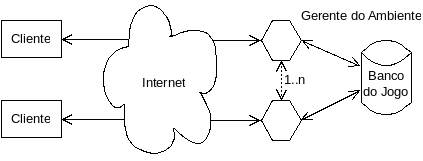
\includegraphics[height=3.5cm]{img/cap3/rudy.png}
  \centering

  Adaptado de:~\cite{matthiasrudy2011}.
\end{figure}

O banco de dados de armazenamento de estado de mundo é compartilhado na arquitetura Rudy (Figura~\ref{rudy}), porém pode não ter ligação lógica entre cada mundo no banco.
%
Esta arquitetura é escalável, porém é limitada o número de conexões em um único ambiente.



O gerente de ambiente por sua vez será comunicado via \ac{tcp}.
%
O funcionamento interno desta arquitetura trabalhará em rodadas.
%
Cada jogador pode enfileirar somente um número determinado de requisições para ser consumido pelo ciclo de processamento do gerente de ambiente.
%
Por sua vez, o consumidor de requisições irá atualizar o estado no mundo e enviar o resultado, caso a requisição tenha uma resposta.
%
Ele pode ser visualizado na Figura~\ref{fig:processamento}.

Este modelo de processamento paralelo perpetua na arquitetura Willson (Seção~\ref{willson}) e Salz (Seção~\ref{salz}).


\subsection{Willson}
\label{willson}

A arquitetura Willson~\cite{stephenclarkewillson2017}.

\subsection{Salz}
\label{salz}

A arquitetura Salz~\cite{albion_online_unite}.

\section{Critérios de análise}
\label{analise}

\section{Plano de testes}
\label{testes}
